\section{Theoretical Analysis}
\label{sec:analysis}

In this section, the circuit shown in Figure~\ref{fig:circuit_t1} is analysed
theoretically, in terms of its time and frequency responses.

\section{Time response}

The circuit consists of a single V-R-C loop where a current $i(t)$ circulates. The
voltage source $v_I(t)$ drives its input, and the output voltage $v_O(t)$ is taken from
the capacitor terminals. Applying the Kirchhoff Voltage Law (KVL), a single
equation for the single loop in the circuit can be written as

MESH EQUATIONS
\input{mesh_eq_tab}

NODAL EQUATIONS
\input{nodal_eq_tab}

%\begin{figure}[h] \centering
%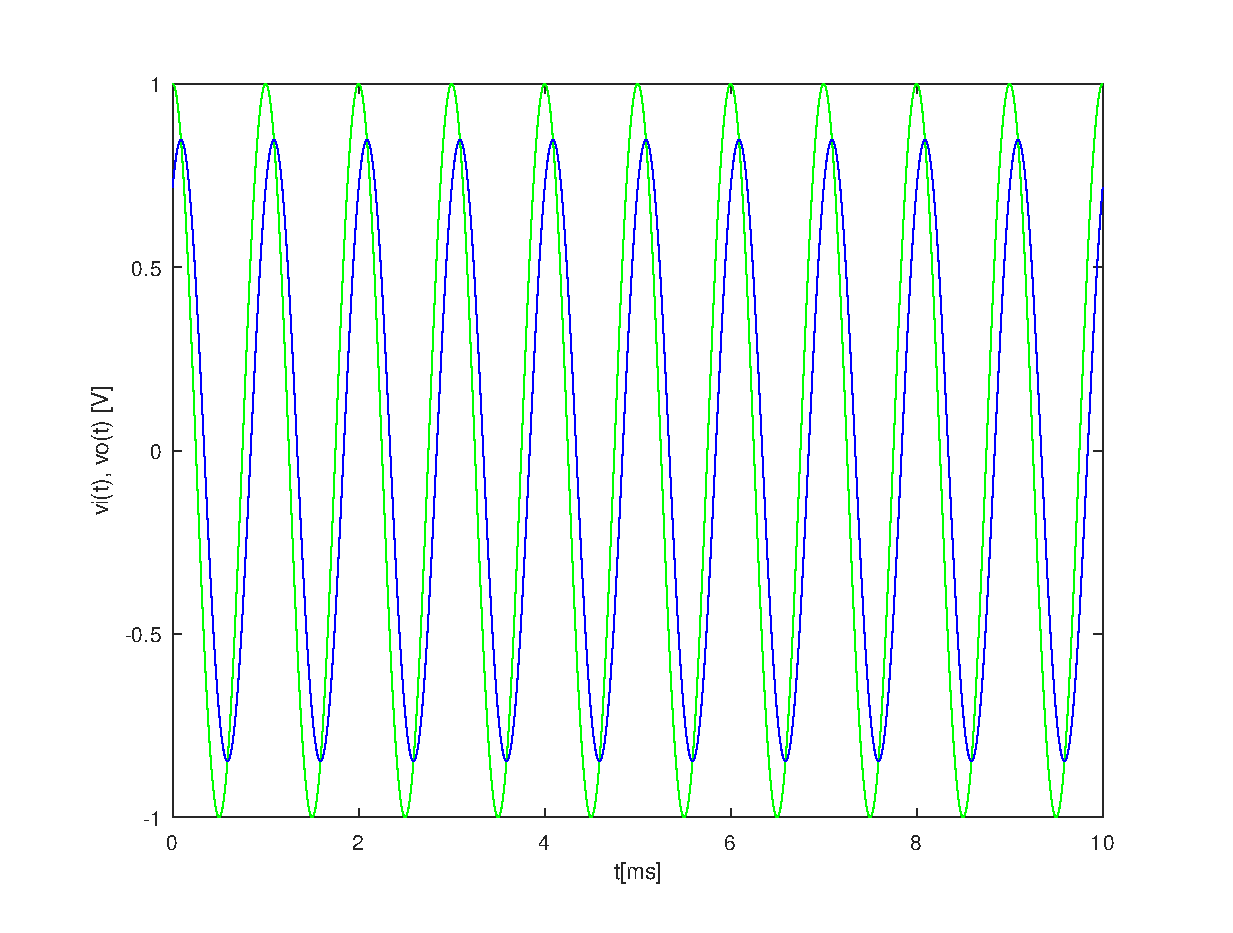
\includegraphics[width=0.8\linewidth]{forced.eps}
%\caption{Forced sinusoidal response.}
%\label{fig:forced}
%\end{figure}

\section{Frequency response}
\begin{table}[h]
  \centering
  \begin{tabular}{|l|r|r|}
    \hline    
    {\bf Name} & {\bf Mesh method} & {\bf Node method}\\ \hline
    @Gb & -0.291567 & -0.291567 \\ \hline
@id & 1.018915 & 1.018915 \\ \hline
@r1 & -0.278049 & -0.278049 \\ \hline
@r2 & -0.291567 & -0.291567 \\ \hline
@r3 & -0.013518 & -0.013518 \\ \hline
@r4 & 1.226887 & 1.226887 \\ \hline
@r5 & 1.310482 & 1.310482 \\ \hline
@r6 & -0.948838 & -0.948838 \\ \hline
@r7 & -0.948838 & -0.948838 \\ \hline
V1 & 5.243596 & 5.243596 \\ \hline
V2 & 4.952740 & 4.952740 \\ \hline
V3 & 4.367469 & 4.367469 \\ \hline
V4 & 4.994112 & 4.994112 \\ \hline
V5 & 9.086122 & 9.086122 \\ \hline
V6 & -2.926767 & -2.926767 \\ \hline
V7 & -1.963402 & -1.963402 \\ \hline
V8 & -1.963402 & -1.963402 \\ \hline

  \end{tabular}
  \caption{A variable preceded by @ is of type {\em current}
    and expressed in milliampere (mA); other variables are of type {\it voltage} and expressed in
    Volt (V).}
  \label{tab:theoretical}
\end{table}


